\chapter{Application User Interface }

\label{Chapter6_appUI} 

\begin{comment}
-------------------------------------------------
%								Chapter layout
6. Application User Interface 
	a. Main Layout
		i. Creating or Loading User
		ii. Saving User Data
		ii. Visual Rotation of Gesture
		iv. Adding a New Gesture
	d. Tabular Display of Data
	e. Writing and Reading from CSV
	f. Artifacts and Distribution
		i. Leap App Store
		ii. IDE Build Process and Batch Script
-------------------------------------------------
figures needed:

homescreen,
analyze screen.
load folder button clicked. opened dialog. 
save to csv opened dialog
load/create new user screen. 
load/create new user screen. (with dropdown showing)
testing screen
testing screen after rotation done. also showing user hand. 
savingData popup. 
table with editing in progress. 
creating new gesture

\end{comment}


In this chapter some of the useful UI features of the application will be discussed. 

%------------------------------------------------
%	SECTION 0 Main Layout
%------------------------------------------------
\section{Main Layout}

The application has three main scenes. The first one is the home screen which shows buttons to take the user to the other two scenes; "Enter Test Mode" button takes the user to the scene which is used for collecting data, and "Analyze Data" button takes the user to a scene that allows him/her to view the collected data \parencite{theKey}. The home screen also contains two radio buttons to allow the user to select which hand (left or right) he/she will be testing with the gestures. Figure  \ref{fig:homeScreen} shows the layout of the home screen. 
\begin{figure}[H]
\centering
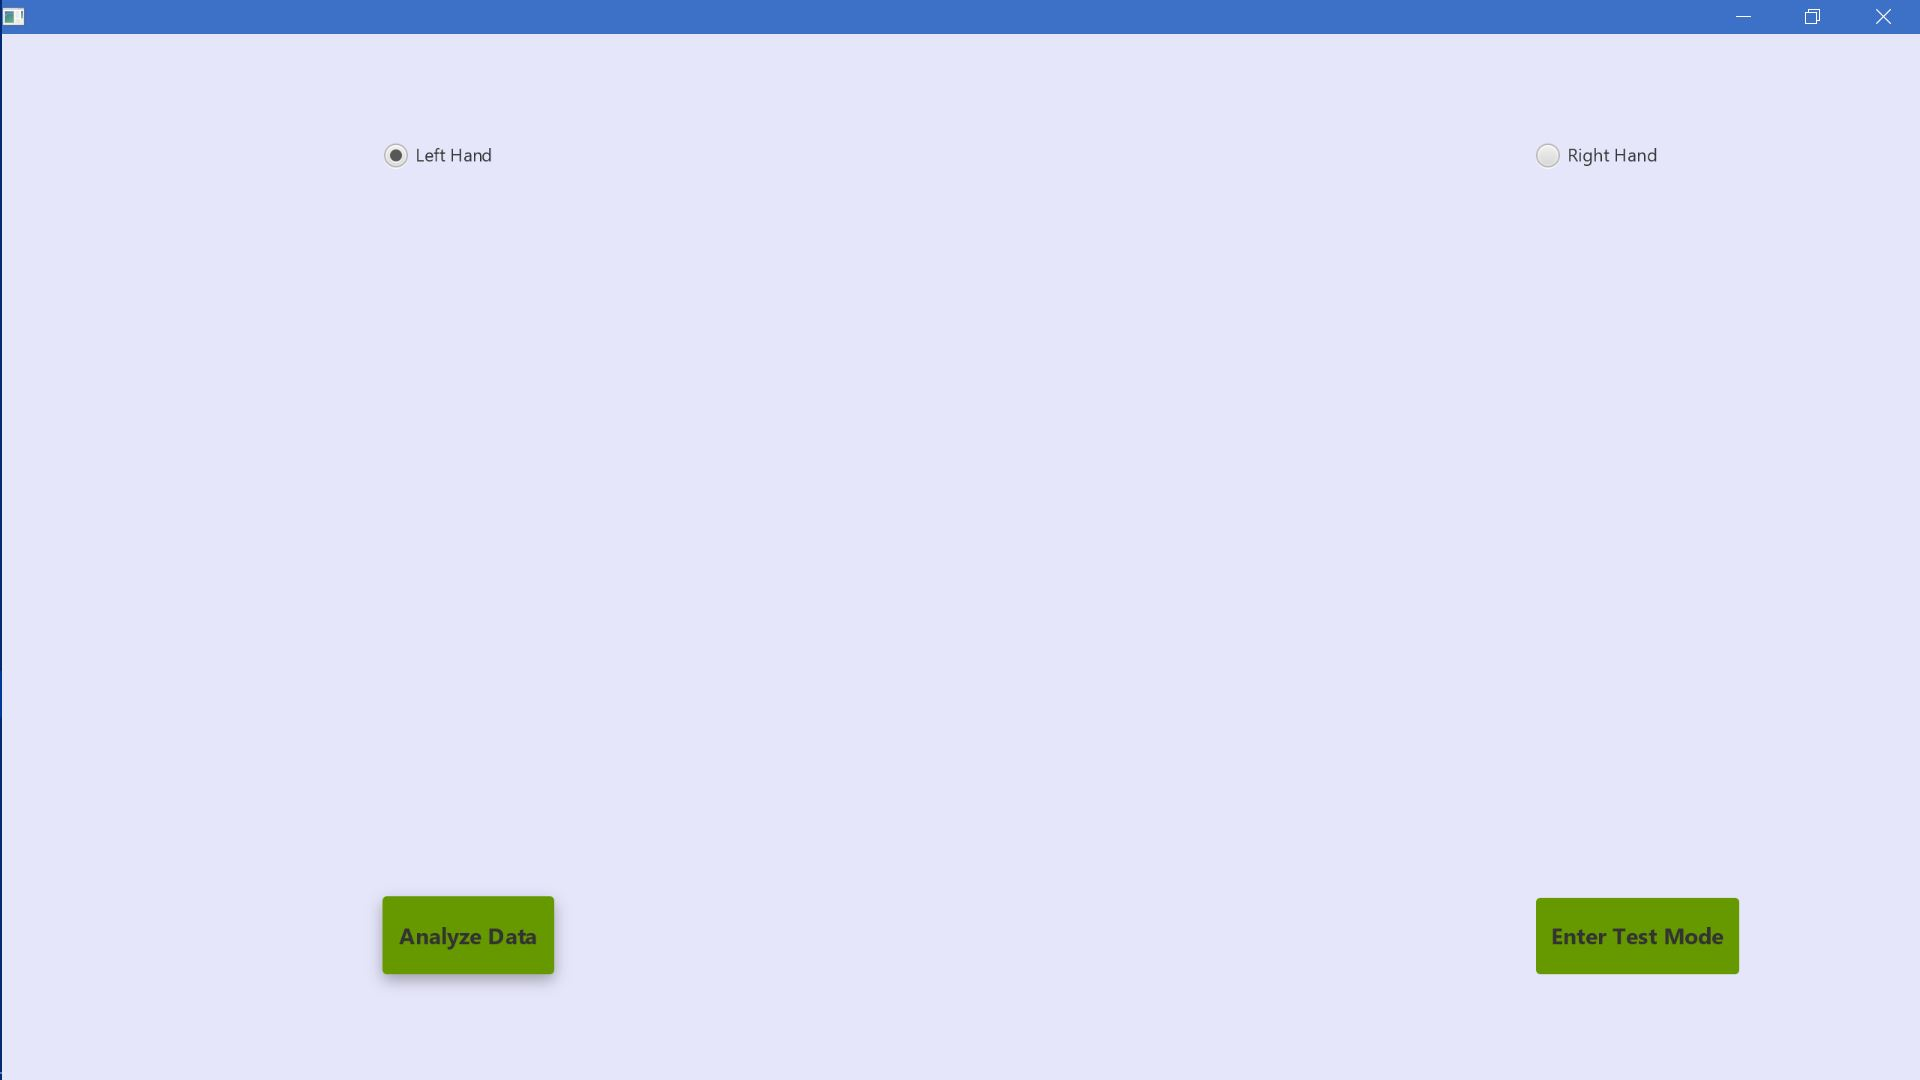
\includegraphics[scale=0.35]{Figures/6_homeScreen.JPG}
\caption[Home Screen Layout]{The scene that the user sees initially when they load the application.}
\label{fig:homeScreen}
\end{figure}


%----------------------------------- Creating or Loading User
\subsection{Creating or Loading User}
The user can click on the "Enter Test Mode" to go to the scene where data will be collected. However, before the user can go to the data collection scene, they must first select a previously saved user or create a new user. All of the hand gesture data collected will be stored in an appropriately named folder for the user. Therefore, when the user clicks on the "Enter Test Mode" the first thing that comes up is a small pop-up screen that asks whether the user would like to create a new user or select an older user; see Figure \ref{fig:createNewUser} and Figure \ref{fig:selectOldUser}. 
\begin{figure}[H]
    \centering
    \begin{minipage}{0.5\textwidth}
        \centering
        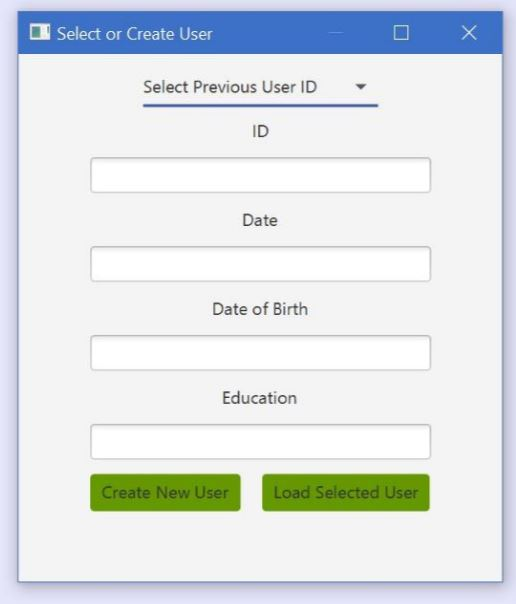
\includegraphics[scale=.55]{Figures/6_selectUser.JPG} 
        \caption{Pop-up window showing options to create or select user. }
		\label{fig:createNewUser}
    \end{minipage}\hfill
    \begin{minipage}{0.5\textwidth}
        \centering
        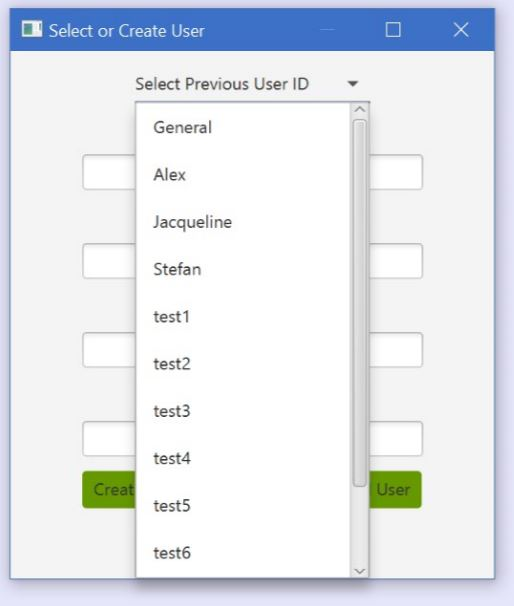
\includegraphics[scale=.55]{Figures/6_selectUserDropdown.JPG}%note png, lower case
        \caption{Pop-up window showing the previously created users.}
        \label{fig:selectOldUser}
    \end{minipage}
\end{figure}
%talk about user object and loading users from file. 
The users shows in the dropdown menu are loaded from a CSV file which is used to record them. Whenever a user is created, a new entry is added to the CSV file for that user. As can be expected these operations are handled by using a convenient User class which encapsulates all the data associated with such an object. 

%----------------------------------- Saving User Data
\subsection{Saving User Data}
After having created or selected a user, the user is taken to the screen where he/she can start to proceed to practicing the ten gestures shown for whichever left/right hand was selected on the home screen; see Figure \ref{fig:dataCollectionScene}. On this data collection screen there are five buttons: the Next and Previous buttons cycle through the gestures, the Save button saves the currently being displayed user hand, the "End Testing" button goes back to the home screen, and the Rotate button which rotates the user and target hand a full 360 degrees slowly.
\begin{figure}[H]
\centering
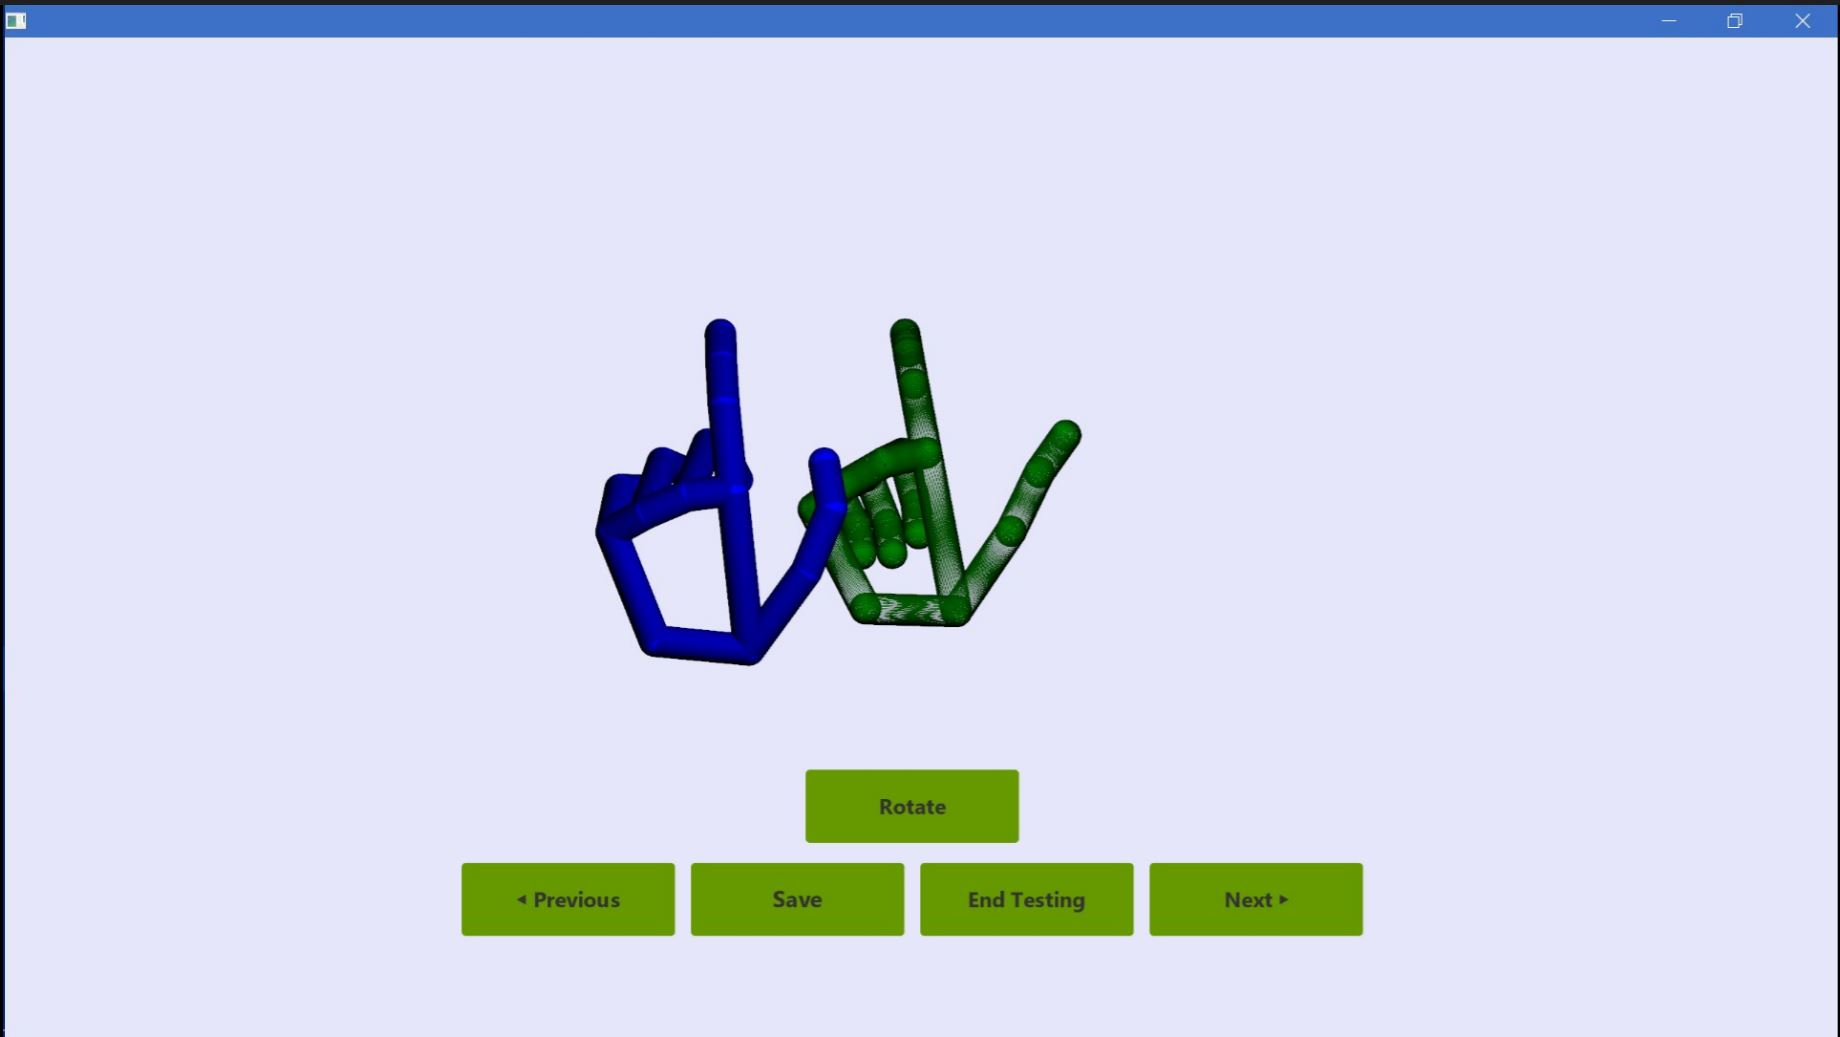
\includegraphics[scale=0.35]{Figures/6_userTargetHand.JPG}
\caption[Data Collection Scene]{This scene is where the user can complete the shown gestures on the screen and the clinicians can collect the user's gesture data.}
\label{fig:dataCollectionScene}
\end{figure}
There are also some keyboard shortcuts that were coded that function in place of some of the buttons. For example, left and right arrows are mapped to the Previous and Next buttons, while the Enter key is mapped to causing the Save Gesture dialog window to pop up just as the Save button does. The user's hand will appear in full blue color on the screen, whereas the target hand the user is trying to imitate will appear in a dark green mesh material. The user's hand will be saved correctly regardless of whether it is exactly covering the target hand. The target hand is just there to give the user indication of the gesture he/she is doing. Figure \ref{fig:saveGestureDialog} shows the Save Gesture dialog which allows the clinicians to type some comments and mark the result of the user's attempt in replicating the shown gesture. 
\begin{figure}[H]
\centering
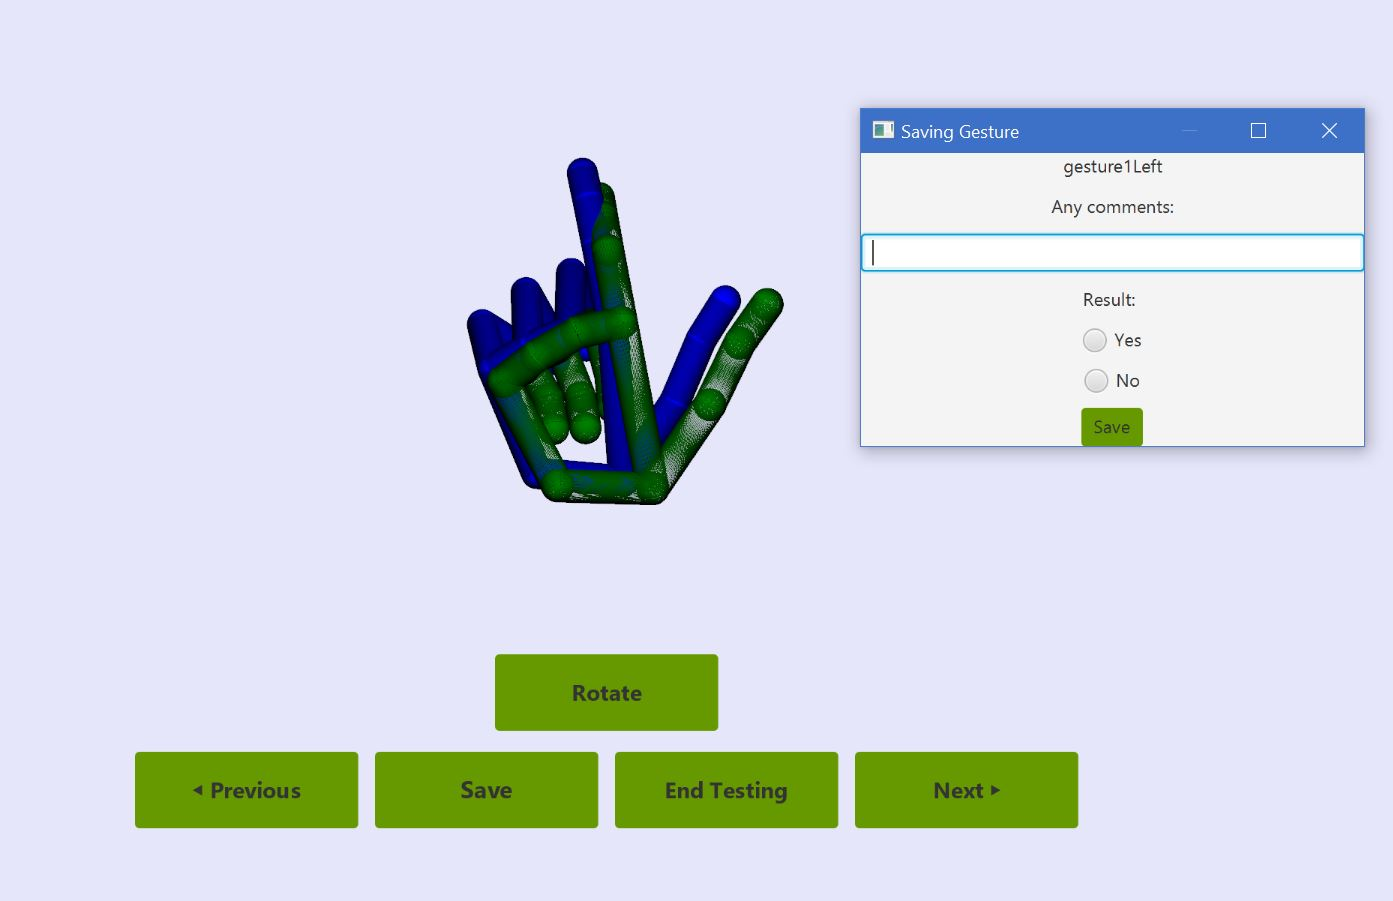
\includegraphics[scale=0.35]{Figures/6_saveGestureDialog.JPG}
\caption[Save Gesture Dialog]{This dialog lets the clinicians grade and comment on the user's gesture before saving it.}
\label{fig:saveGestureDialog}
\end{figure}
By default the result is saved to be "Yes" which indicates the user successfully completed the gesture. In the code, there is an object called HandInfo which represents the data being saved including the full file path of where the Leap Motion Hand object will be serialized to, and the comments and the result of the gesture attempt. 

%----------------------------------- Visual Rotation of Gesture
\subsection{Visual Rotation of Gesture}
The Rotate button causes the 3D camera that is being used in the application to spin around. The user and target hands themselves do not move at all, it is the camera that orbits around them while being focused on them. A picture taken while the rotation was happening is shown in Figure \ref{fig:rotationButtonDemo}.
\begin{figure}[H]
\centering
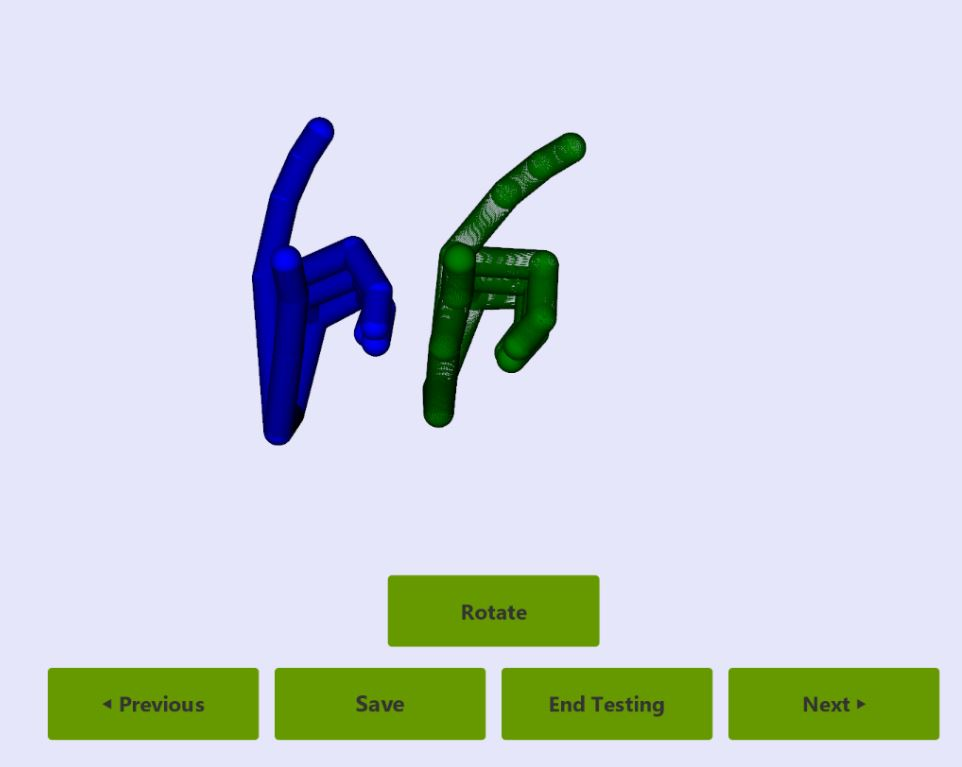
\includegraphics[scale=0.35]{Figures/6_rotationButtonDemo.JPG}
\caption[Rotation Button in Action]{This figure shows instance of the rotation in action. The hands are shown at 90 degree angle because of the camera rotating around them.}
\label{fig:rotationButtonDemo}
\end{figure}

The way this is achieved via code is shown in Figure \ref{fig:visualRotationCode1}. In order for the user to observe the rotation happen in real time on the screen, a Timeline object was used to set up an animation which can update the observable angleProperty() of a rotation transform object  attached to the camera in advance. The timeline was set to last for seven seconds and the starting and ending angles were 0 and 360 degrees respectively. The code which actually initializes and adds the Rotate transform to the 3D perspective camera of the application is shown in Figure \ref{fig:visualRotationCode2}. 
\begin{figure}[H]
\centering
\begin{lstlisting}
//set up rotation timeline
Timeline timeline = new Timeline(
	new KeyFrame(Duration.seconds(0), new KeyValue(rotateAroundY.angleProperty(), 0)),
	new KeyFrame(Duration.seconds(7), new KeyValue(rotateAroundY.angleProperty(), -360)));
timeline.setCycleCount(1);
... 
//rotate button plays animation
rotateButton = new Button("Rotate") {
	@Override
	public void fire() {
	timeline.play();}
};
\end{lstlisting}
\caption[Rotation Animation Timeline]{This code shows the Timeline object that was used to animate the movement of the 3D camera around the y-axis.}
\label{fig:visualRotationCode1}
\end{figure}
Since the "rotateAround" transform object is added first to the camera's transforms, it will be the last transform to be executed. This is exactly what we want so the camera will remain focused on the hands as it rotates. 
\begin{figure}[H]
\centering
\begin{lstlisting}
// The 3D camera
PerspectiveCamera camera = new PerspectiveCamera(true);
// The rotation transform to be updated later
rotateAroundY = new Rotate(0, Rotate.Y_AXIS);
// rotation transform is added first. It will be executed last
camera.getTransforms().addAll(rotateAroundY, new Translate(0, -5, -50), new Rotate(-10, Rotate.X_AXIS));
\end{lstlisting}
\caption[Rotation Transform on Camera]{This code shows the rotate transform that's added to the camera. This transform gets updated by the animation timeline object.}
\label{fig:visualRotationCode2}
\end{figure}

The hands themselves are not affected at all by the rotation and in fact during the seven seconds in which the camera is being rotated around the y-axis, the user can continue trying to imitate the gesture. However, during testing of the application it was found out that most users prefer to have to rotation happen in separately initially so they can just observe. Only after the rotation finishes is when they would start trying to perform the gesture. 
	
%----------------------------------- Adding a New Gesture
\subsection{Adding a New Gesture}
From the data collection scene page, it is also possible to create a new target gesture and add it to the stock of target gestures being considered. This functionality was not really required by the clinicians, however it did come in useful when I was developing the application and it does have the potential of becoming a useful feature if the application is ever deployed into a real life environment. Currently the application interface does not have a button the user or clinicians can press to bring up the Save Gesture dialog window. Instead, there is a keyboard command that is listened for in the code and which is triggered by pressing the letter "G". This brings up the Save Gesture dialog, a picture of which is shown in Figure \ref{fig:saveGesture}. 
\begin{figure}[H]
\centering
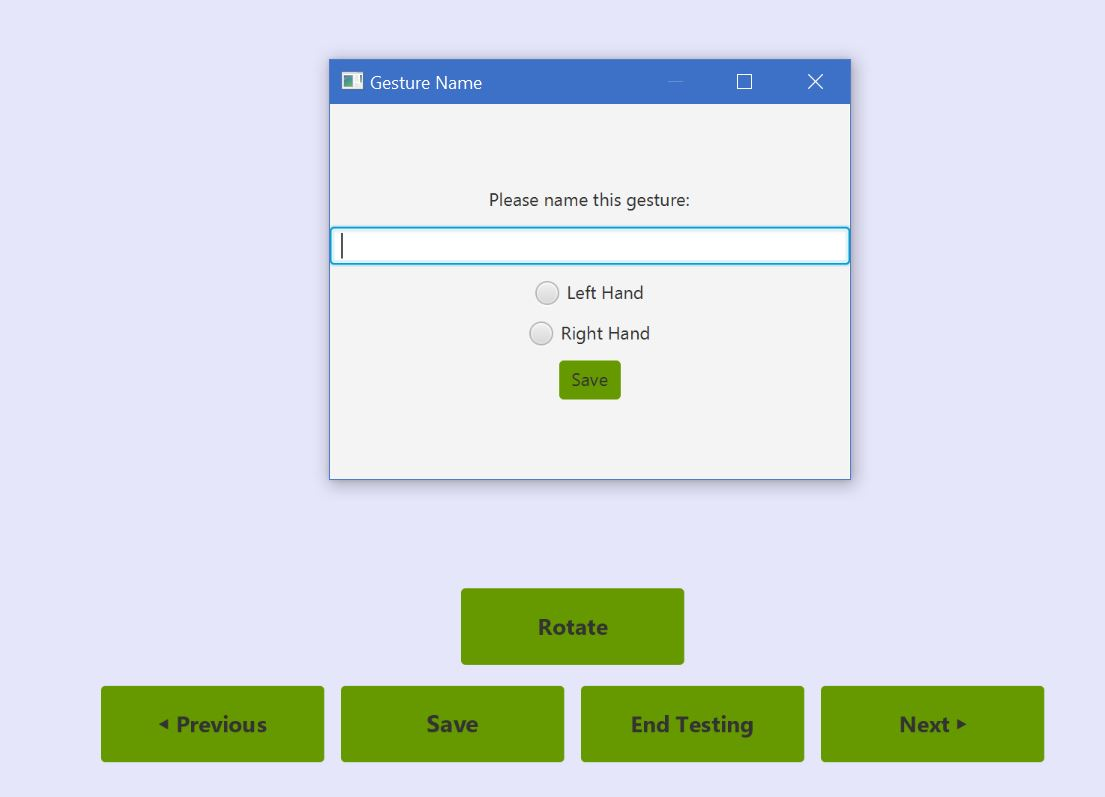
\includegraphics[scale=0.45]{Figures/6_createNewGesture.JPG}
\caption[Saving New Gesture]{This dialog window will save the current user hand as a new gesture, in the list of target gestures.}
\label{fig:saveGesture}
\end{figure}
Saving a new gesture will add it to the end of the list of currently used gestures. 

%------------------------------------------------
%	SECTION 3 Tabular Display of Data
%------------------------------------------------
\section{Tabular Display of Data}
If the user clicks on the "Analyze Data" button on the home screen, he/she will be taken to a scene shown in Figure \ref{fig:analyzeData}. This scene shows all of the collected data for the currently selected user in a table on the left. The user is able to select rows in the table by pressing the Up or Down keys on the keyboard or by clicking on a row with their mouse. 
\begin{figure}[H]
\centering
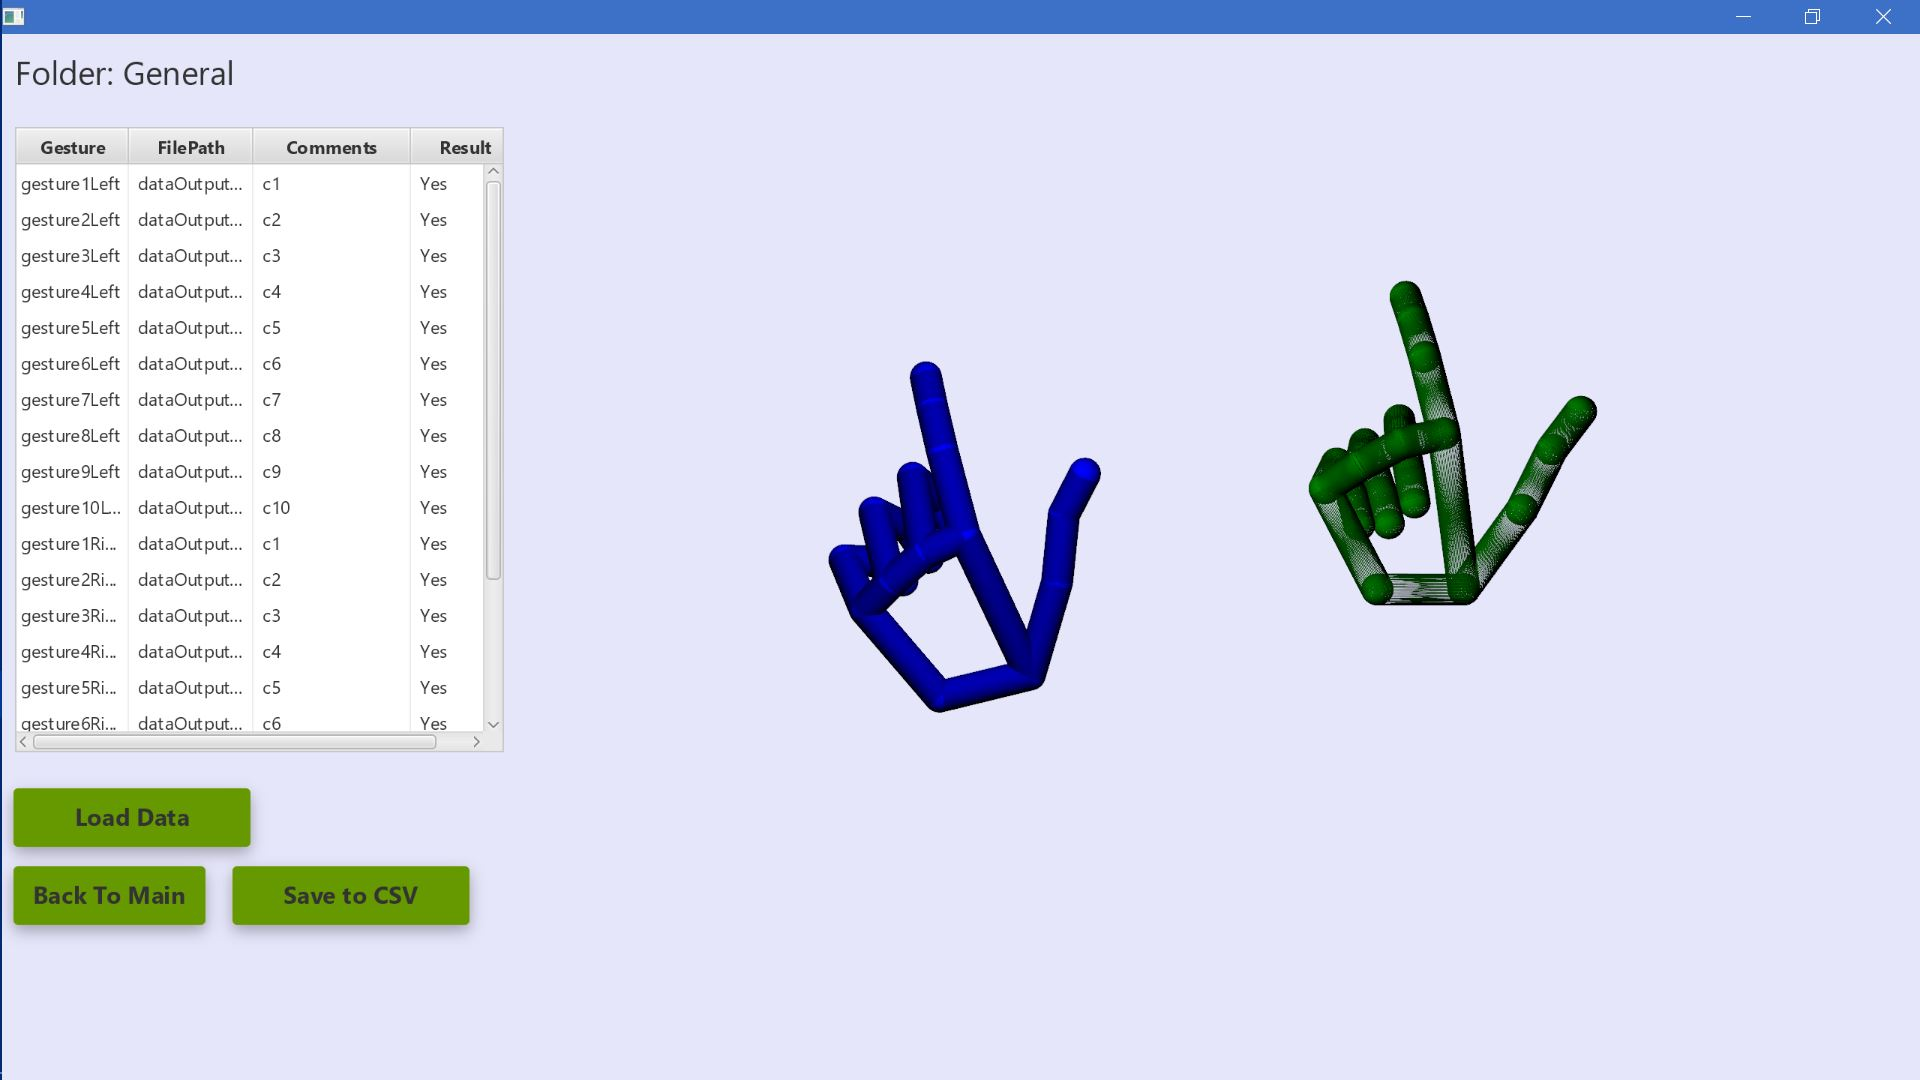
\includegraphics[scale=0.45]{Figures/6_analyzeScreen.JPG}
\caption[Analyze Data Scene]{The scene which allows user to view and edit some of the meta-data on the hand objects saved for the currently loaded user.}
\label{fig:analyzeData}
\end{figure}
This table is sortable by the columns and the columns can also be rearranged to be in a different order. In addition, some of the columns are actually editable and allow the user to specify changes to the data recorded. These changes will be updated for the user when the application is closed or the user navigates to a different scene. The way in which this table is constructed and made to be editablee is shown in the snippets of code in Figure \ref{fig:tabularDataCode}. This code is all from the controller Java class that is set for this scene. A part of this scene was built using Scene Builder and part of it was procedurally created using just Java code. The table section was prototyped in Scene Builder and the section of the scene to the right showing the two hands was created in Scene Builder.
\begin{figure}[H]
\centering
\begin{lstlisting}
//bind references with fxml annotations
@FXML
private TreeTableView<HandInfo2> treeTableView;
@FXML
private TreeTableColumn<HandInfo2, String> col3;
...
//set up results column; using lambda function
col3.setCellValueFactory((TreeTableColumn.CellDataFeatures<HandInfo2, String> param) -> param.getValue().getValue().result2Property());
//set up results column to be editable
ObservableList<String> list = FXCollections.observableArrayList();
list.add("Yes");
list.add("No");
col3.setCellFactory(ChoiceBoxTreeTableCell.forTreeTableColumn(list));
col3.setOnEditCommit(new EventHandler<TreeTableColumn.CellEditEvent<HandInfo2, String>>() {
	@Override
	public void handle(TreeTableColumn.CellEditEvent<HandInfo2, String> event) {
		TreeItem<HandInfo2> h = treeTableView.getTreeItem(event.getTreeTablePosition().getRow());
		h.getValue().setResult(event.getNewValue());
	}
});
...
//make table editable
treeTableView.setEditable(true);
\end{lstlisting}
\caption[TreeTableView Editable Results Column]{These sections of code show how the table and a specific column were accessed from the FXML file. The code also shows how the column was set up to be editable by the user.}
\label{fig:tabularDataCode}
\end{figure}







discuss annotation. reference background. --maybe
discuss lambda function. observable property. finish up. why need to be editable. explain use case as discussed with clinicians. comments section later. file path changes. etc. have some good discussion. 




\begin{comment}

editable picture. show code about how table was constructed. maybe even discuss scenebuilder. 

 The user can click on the "Analyze Data" button to go to the 
talk about three scenes and show pics. show what happens where and 
what the typical user would do. 
take data and analyze it for problems. 
and then go fix those problems. 
also save data to csv. read from csv. 
say some things will be dicussed in other sections. 
\end{comment}





%------------------------------------------------
%	SECTION 4 Writing and Reading from CSV
%------------------------------------------------
\section{Writing and Reading from CSV}


%------------------------------------------------
%	SECTION 5 Artifacts and Distribution
%------------------------------------------------
\section{Artifacts and Distribution}

maybe this section can all be collapsed into one. (IDE Build Process and Batch Script)

%----------------------------------- Leap App Store
\subsection{Leap App Store}

%----------------------------------- IDE Build Process and Batch Script
\subsection{IDE Build Process and Batch Script}


